\documentclass{article}
\usepackage[utf8]{inputenc}
\usepackage[ngerman]{babel}
\usepackage{hyperref}
\usepackage{graphicx}

\title{BSRN}
\author{Pascal Lupo, Gammachu Tufa, Jean-Gabriel Hanania}
\date{\today}

\begin{document}

\maketitle
\tableofcontents



\newpage
\part{Einführung}
\part{Aufbau des Spieles}
\section{Main}
\section{Menu}
\section{Game Functions}
\section{Function}
\section{Counter}
\subsection{Aufgabe der Funktion}
\paragraph{Die Funktion ist dafür da, um die Zeit der Benutzereingabe zeitlich zu begrenzen. Sobald der Spieler aufgefordert wir ein gegnerisches Feld zu beschießen,  läuft ein Countdown runter, der aufzeigt wie viel Zeit noch übrig geblieben ist. Wir haben uns dafür entschieden einen Zeitraum von 15 Sekunden festzulegen. Sollte der Spieler innerhalb der gegebenen Zeit ein gegnerisches Schiff beschießen, wird der Countdown beendet und das Spiel fortgesetzt, in dem der andere Spieler nun aufgefordert wird ein gegnerisches Feld zu beschießen. Sollte der Spieler bis Ablauf der Zeit noch kein Feld ausgewählt haben, wird dem Spieler angezeigt, dass seine Zeit abgelaufen ist und er nun die Enter-Taste drücken soll. Durch das Drücken der Enter-Taste wird ein zufälliges Feld beschossen und so dass, das Spiel fortgesetzt.
Diese Funktion wird jedes Mal aufgerufen, wenn der Spieler ein Feld beschießen muss.}
\subsection{Problemstellung}
\paragraph{Ein Problem der Aufgabenstellung war, dass zwei Prozesse gleichzeitig laufen müssen. Zum einen muss der Countdown von 15 bis 0 runterlaufen, zum anderen muss gleichzeitig auf einen Benutzereingabe gewartet werden. Zu beginn hatte ich das Problem, dass der Countdown erst gestartet ist, nach dem es eine Benutzereingabe gab. Dies machte den Countdown jedoch unbrauchbar, da es parallel laufen muss.}
\subsection{Lösungsversuch}
\paragraph{Um nun mehrere Prozesse gleichzeitig laufen zu lassen musste eine andere Lösung her. Durch etwas Recherche fand ich einige Informationen zu "threads". Diese sollten einen parallelen Ablauf von mehreren Prozessen möglich machen. Die Datei ist wie folgt aufgebaut.\\\\Es gibt die ask()-Funktion. Diese Funktion nimm die Benutzereingabe auf und gibt sie später, am Ende zurück.\\Die Funktion exit(msg). Wird aufgerufen, wenn eine Benutzereingabe erfolgt ist oder wenn keine Eingabe erfolgt ist. In beiden Fällen gibt die Funktion einen Textwert zurück, der als Parameter gegeben werden muss. Es wird beispielsweise ausgegeben, dass die Zeit abgelaufen ist und nun ein zufälliges Feld beschossen wird oder es wird ausgegeben, auf welches Feld geschossen wurde.\\Die Funktion countdown() gibt die verbliebene Zeit an. Innerhalb der Funktion ist eine Endlosschleife die läuft, bis der Stop-Wert null erreicht wird. Der Wert beginnt bei 15 und wird  jede Runde, mit einer  Verzögerung von 2 Sekunden um den Wert 2 verringert. Bei jeden Schleifendurchgang wird die aktuell verbliebene Zeit ausgegeben. Wichtig  ist hierbei zusagen, dass in der Gesamten zeit eine Benutzereingabe parallel möglich ist.\\Die Funktion close\_if\_time\_pass(seconds) wird als letztes aufgerufen und gibt aus, dass die Zeit abgelaufen ist.\\Alle diese Funktionen werden in der Wichtigsten von allen, der main() Funktion, aufgerufen.\\\\In der Funktion main(), habe ich, wie bereits erwähnt, mit "threads"\\gearbeitet. Ich habe dazu 2 "threads" erstellt. Der erste ist dafür da, um nach Ablauf der Zeit (in unserem Fall 15 Sekunden) auszugeben, dass die Zeit abgelaufen ist und nun vom Spiel selbst, ein zufälliges Feld ausgewählt wird. Der zweite "thread" ist dazu da, den Countdown zu starten.\\Sobald die "threads" gestartet werden, wird die Funktion ask() aufgerufen, welche auf die Benutzereingabe wartet. Der Rückgabewert aus der Funktion ask(), wird gespeichert in der Variable user\_input. Es wird nach Ablauf der Zeit geprüft, ob die Variable keinen Wert hat. Sollte dies der Fall sein, wird ein zufälliges Feld beschossen, mit der Funktion random\_ship\_attac, aus der Date gamefunctions. Sollte die Variable jedoch einen Wert haben, wird dieser Wert als Rückgabewert genutzt und somit das eingegeben Feld beschossen.  } 



\begin{center}
    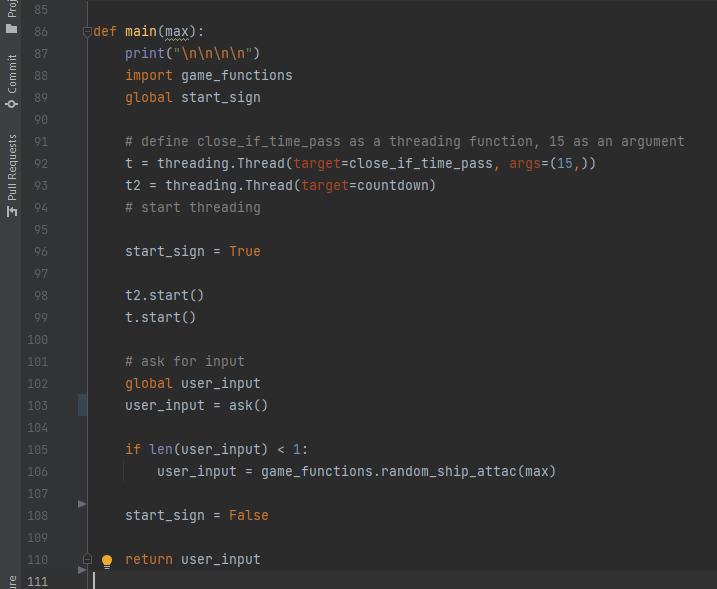
\includegraphics[width=1.20\textwidth]{BSRNScreenshotCounter.png}
\end{center}


\section{Languages}
\section{Zufalls Generator}
\section{PvE Game}
\subsection{Aufbau des PvE}
\paragraph{Der PvE Modus ist dafür da, dass eine Person gegen einen Bot spielen kann. In diesem Modus kann man außerdem auswählen, ob der Bot mit einer hohen KI oder einer geringen KI ausgestattet werden soll. Diese Einstellung, kann einen sehr guten Gegenspieler oder einen weniger gute Spieler imitieren, was das allgemeine Spielerlebnis abwechslungsreicher macht.}
\subsection{Probleme bei der Umsetzung}
\paragraph{Einer der größten Probleme bei der Umsetzung des PvE Modus war es die KI zu integrieren, als Beispiel: Soll der Bot auf die umliegenden Felder schießen, wenn er ein Schiff getroffen hat und nicht einfach weiter zufällig auf das gegnerische Spielfeld schießen.}
\subsection{Lösungen}
\paragraph{Bei der Umsetzung gab es auch einige Probleme, es war ziemlich kompliziert die einzelnen Schwierigkeitsgrade einzubauen. Die Lösung war am Ende,dass der Bot im  Easy Modus komplett zufällig schießt. Und im Normal Modus der Bot auf die Umliegenden Felder schießt falls der letzte Schuss ein Treffer war, bis das Schiff versenkt ist.}

\section{PvP Game}
\subsection{Aufbau des PvP Modus}
\paragraph{Beim PvP Modus, ist es möglich, dass 2 Personen an einem Gerät gegeneinander spielen können. In dem Modus können beide Spieler einen Namen auswählen und werden daran erinnert, dass sie auf den Bildschirm schauen sollen, wenn der gegen Spieler an der Reihe ist. Der Spieler selbst kann auch auswählen, ob seine Schiffe zufällig gesetzt werden sollen oder ob er sie selbst platzieren will.}
\section{Drawing Utils}
\end{document}


